\begin{figure*}[h!]
\centering
\vspace{-10pt}
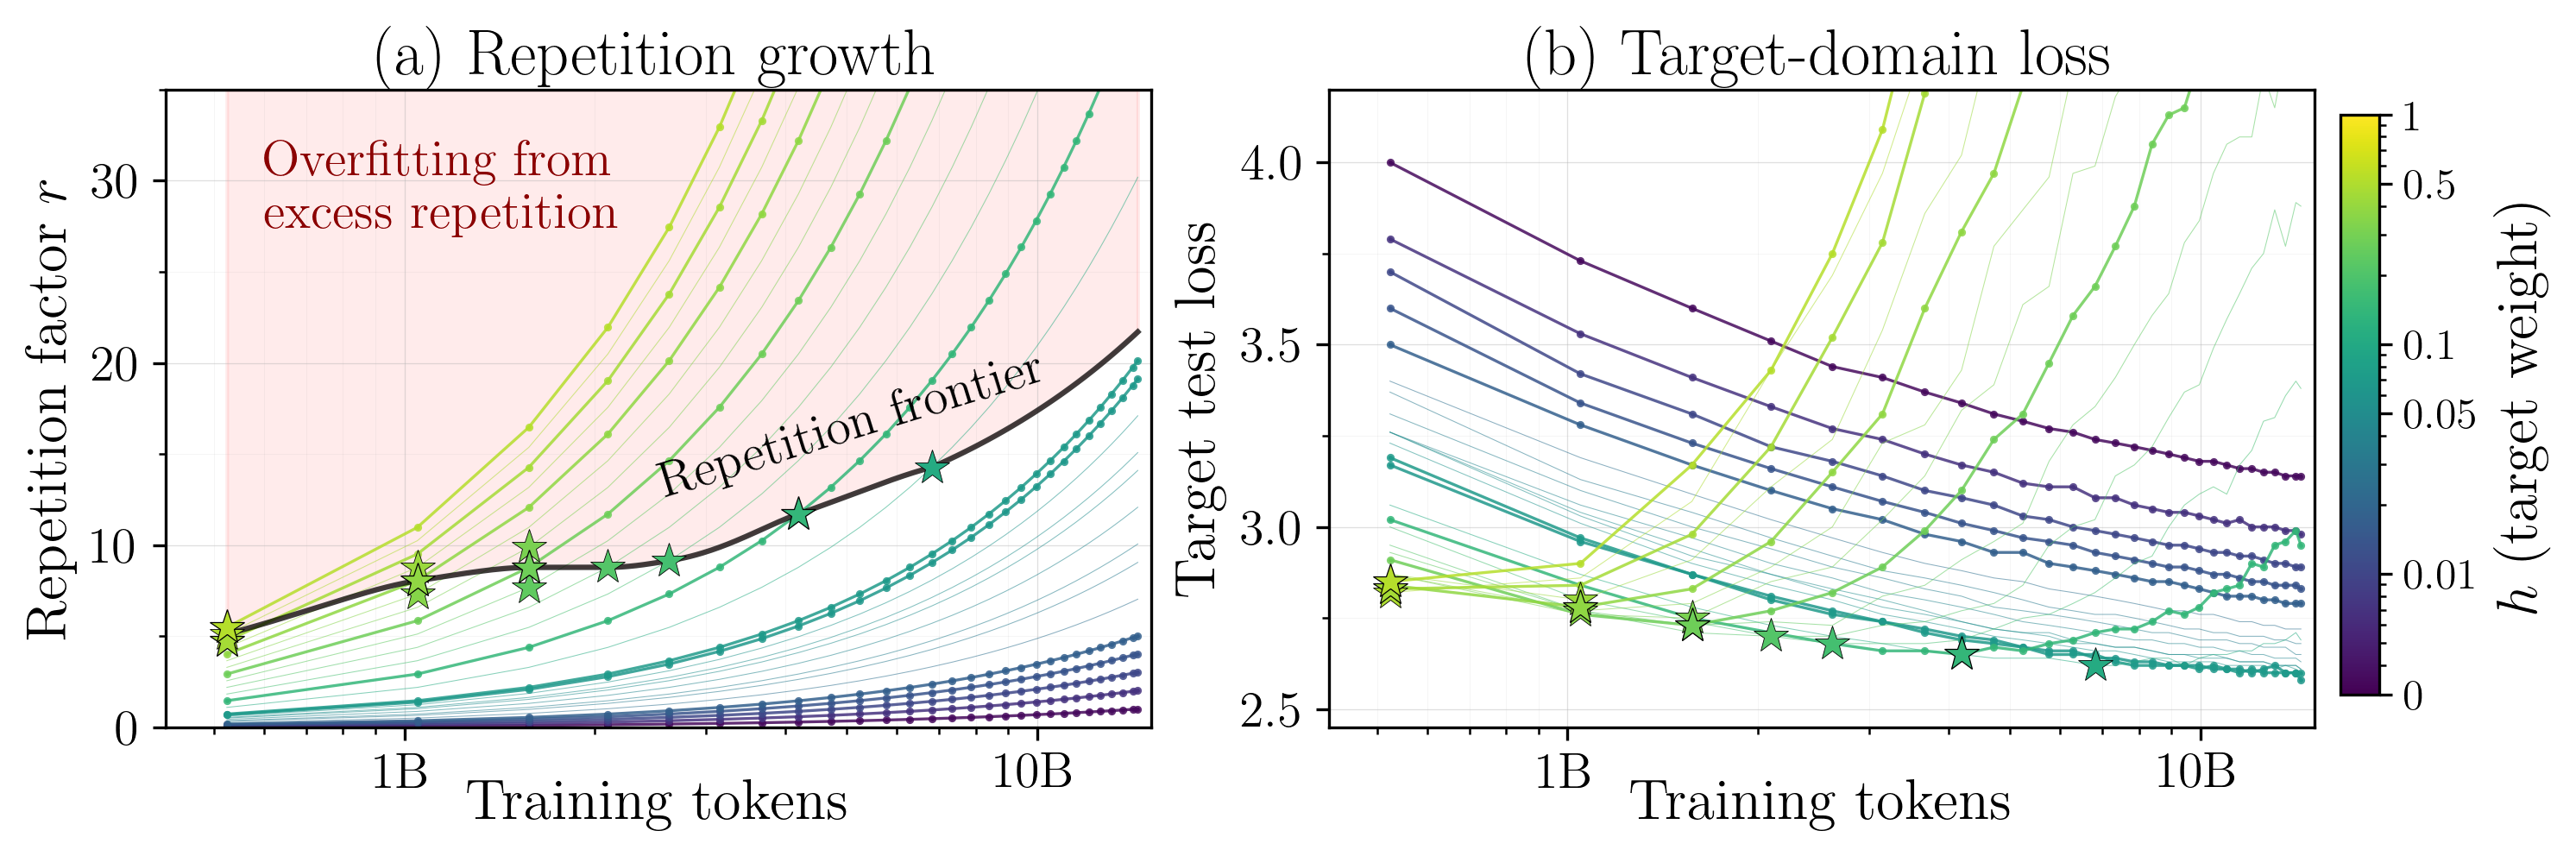
\includegraphics[width=0.82\textwidth]{figures/fig_main_dual_frontier_clean.png}
\vspace{-5pt}
\caption{Repetition dynamics for 143M model, 50M German tokens mixed with English, $h$ defining the weight of German data in the training mix.
\textbf{(a)}~Repetition factor $r$ grows with training tokens; beyond the repetition frontier, loss begins to increase. \textbf{(b)}~German validation loss vs.\ training tokens. Stars indicate overfitting onset.}
\vspace{-10pt}
\label{fig:main}
\end{figure*}
\section{Introduction}
Large language models (LLMs) have demonstrated remarkable performance across a wide range of language understanding, mathematics, science, and knowledge-intensive tasks \citep{luong2025advanced,woodruff2026accelerating,singh2025openai,antropic2026}. 
While much of this success can be attributed to large scale pretraining corpora exceeding trillions of tokens \citep{hojel2025essential,li2024datacomp}, many language model pretraining scenarios involve data that cannot be freely scaled including low-resource languages, specialized domains, and curated datasets, which offer far less unique data.
During pretraining, this data is mixed with abundant generic data, such as pairing low-resource language text with English text, or a domain-specific math corpus with generic web text.

\begin{wrapfigure}{r}{0.4\textwidth}
\centering
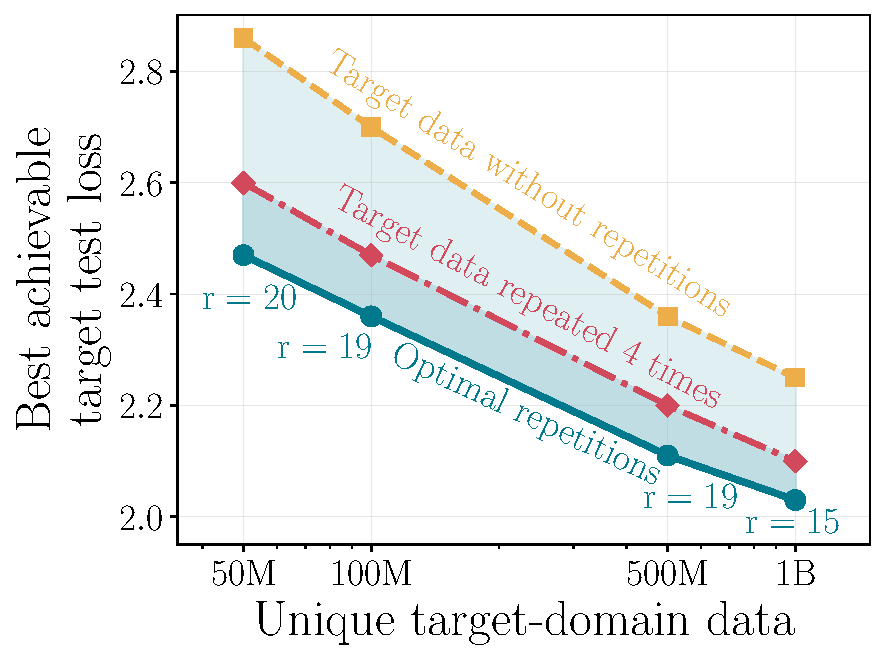
\includegraphics[width=0.4\textwidth]{figures/fig_diminishing_returns_539M}
\vspace{-15pt}
\caption{Best achievable German test loss by target data size, shown for the 539M model.}
\label{fig:diminishing_539M}
\vspace{-5pt}
\end{wrapfigure}

However, mixing introduces a new trade-off. The limited data must be repeated for enough of the total training to provide sufficient target-domain signal, but high repetition leads to memorization and eventual overfitting. Figure~\ref{fig:main} illustrates this challenge for a 143M model with 50M German tokens mixed with English. Higher fractions of German data start overfitting (Figure~\ref{fig:main}b) as the number of repetitions crosses a frontier (Figure~\ref{fig:main}a).
This raises the question: \textit{how do model scale, data size, and repetition jointly shape the outcome of mixture pretraining when target data in the mixture is constrained?}

Prior work has studied these two dimensions separately. 
\citet{muennighoff2023scaling} derive scaling laws for data-constrained training, showing that up to 4 repetitions over a fixed monolithic dataset are nearly as valuable as unique data.
However, this result, widely adopted as a practical ceiling for data repetition, applies to single-source training where \emph{all} tokens are repeated.
In mixture pretraining, only the constrained domain is repeated while the generic domain continues to supply fresh tokens, which is a structurally different regime.
Conversely, data mixing laws \citep{ye2024data, xie2024doremi, shukor2025scalinglawsoptimaldata} optimize the composition of training mixtures to maximize downstream performance, but assume each data source has unlimited data.
Our work sits at the intersection: we study how to optimally mix data-constrained sources with abundant ones, jointly optimizing mixture weights and repetition, a setting that arises in many real-world pretraining scenarios.

Our contributions are:
\begin{itemize}[leftmargin=1.5em]
    \item A systematic empirical study of over 2000 training runs spanning model sizes from 101M to 805M parameters, different target data sizes, and diverse data types: multilingual (German, French, Swahili), multi-domain (mathematics, scientific papers, Wikipedia), and quality-filtered subsets.
    \item Empirical findings on repetition in data mixtures: repeated tokens follow diminishing returns predictably across all data types; optimal repetition scales with target dataset size and compute budget; and larger models consistently extract more from limited data despite overfitting faster. 
    Crucially, abundant generic data sustains learning and unlocks far higher repetition than
    reported for single-source training without performance degradation, with optimal for target task performance repetitions reaching 15-20 times (Figure~\ref{fig:diminishing_539M}).
    \item A scaling law at the intersection of data-constrained training and mixture optimization that predicts target-domain loss as a function of target data size, mixture ratio, and model size. We demonstrate that this scaling law can be fitted at small scales and then extrapolates at larger scales, and that it can be used to estimate accurately the optimal number of repetitions.
\end{itemize}


We also extend our findings to the case of two scarce target domains.
Together, our findings provide both empirical understanding of how repetition behaves in data mixtures and a predictive scaling law for training effectively on limited target data.
